\documentclass{article}
\usepackage{graphicx}
\usepackage{subcaption}
\usepackage{caption}

\begin{document}

\begin{figure}[htbp]
    \centering
    \begin{subfigure}{0.45\textwidth}
        \centering
        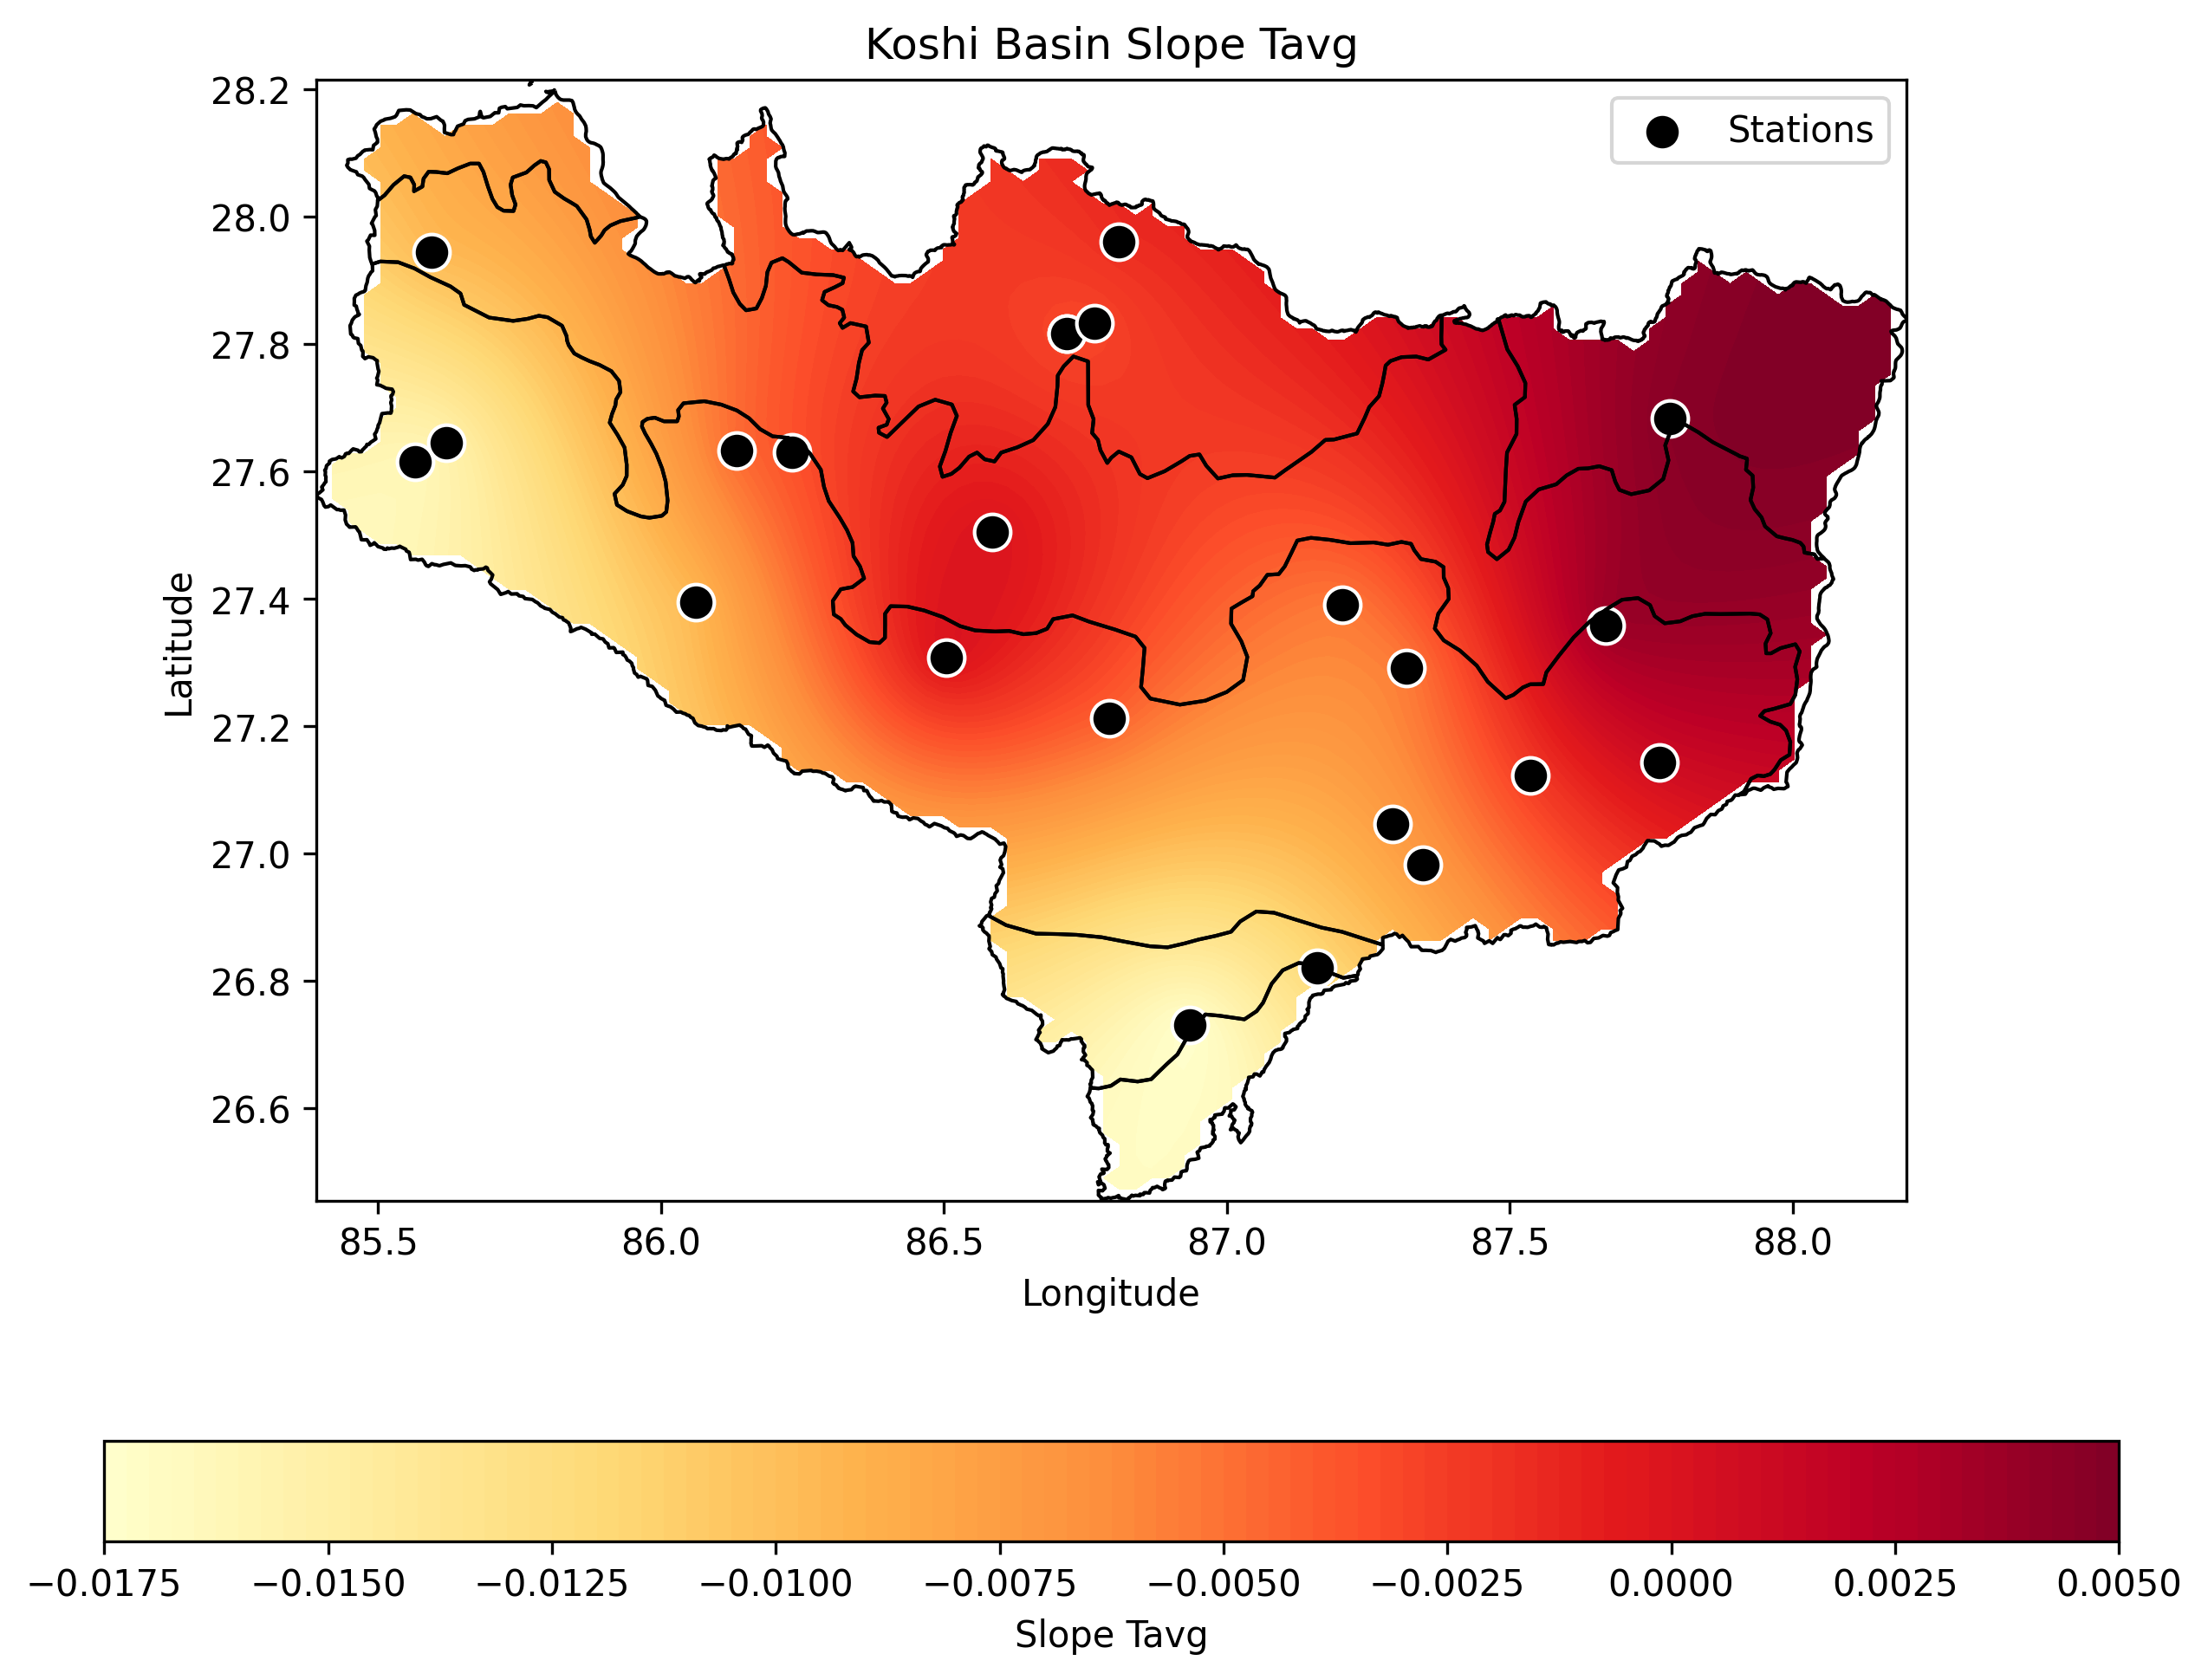
\includegraphics[width=\linewidth]{figure1.png}
        \caption{Caption for subfigure (a)}
        \label{fig:7a}
    \end{subfigure}
    \hfill
    \begin{subfigure}{0.45\textwidth}
        \centering
        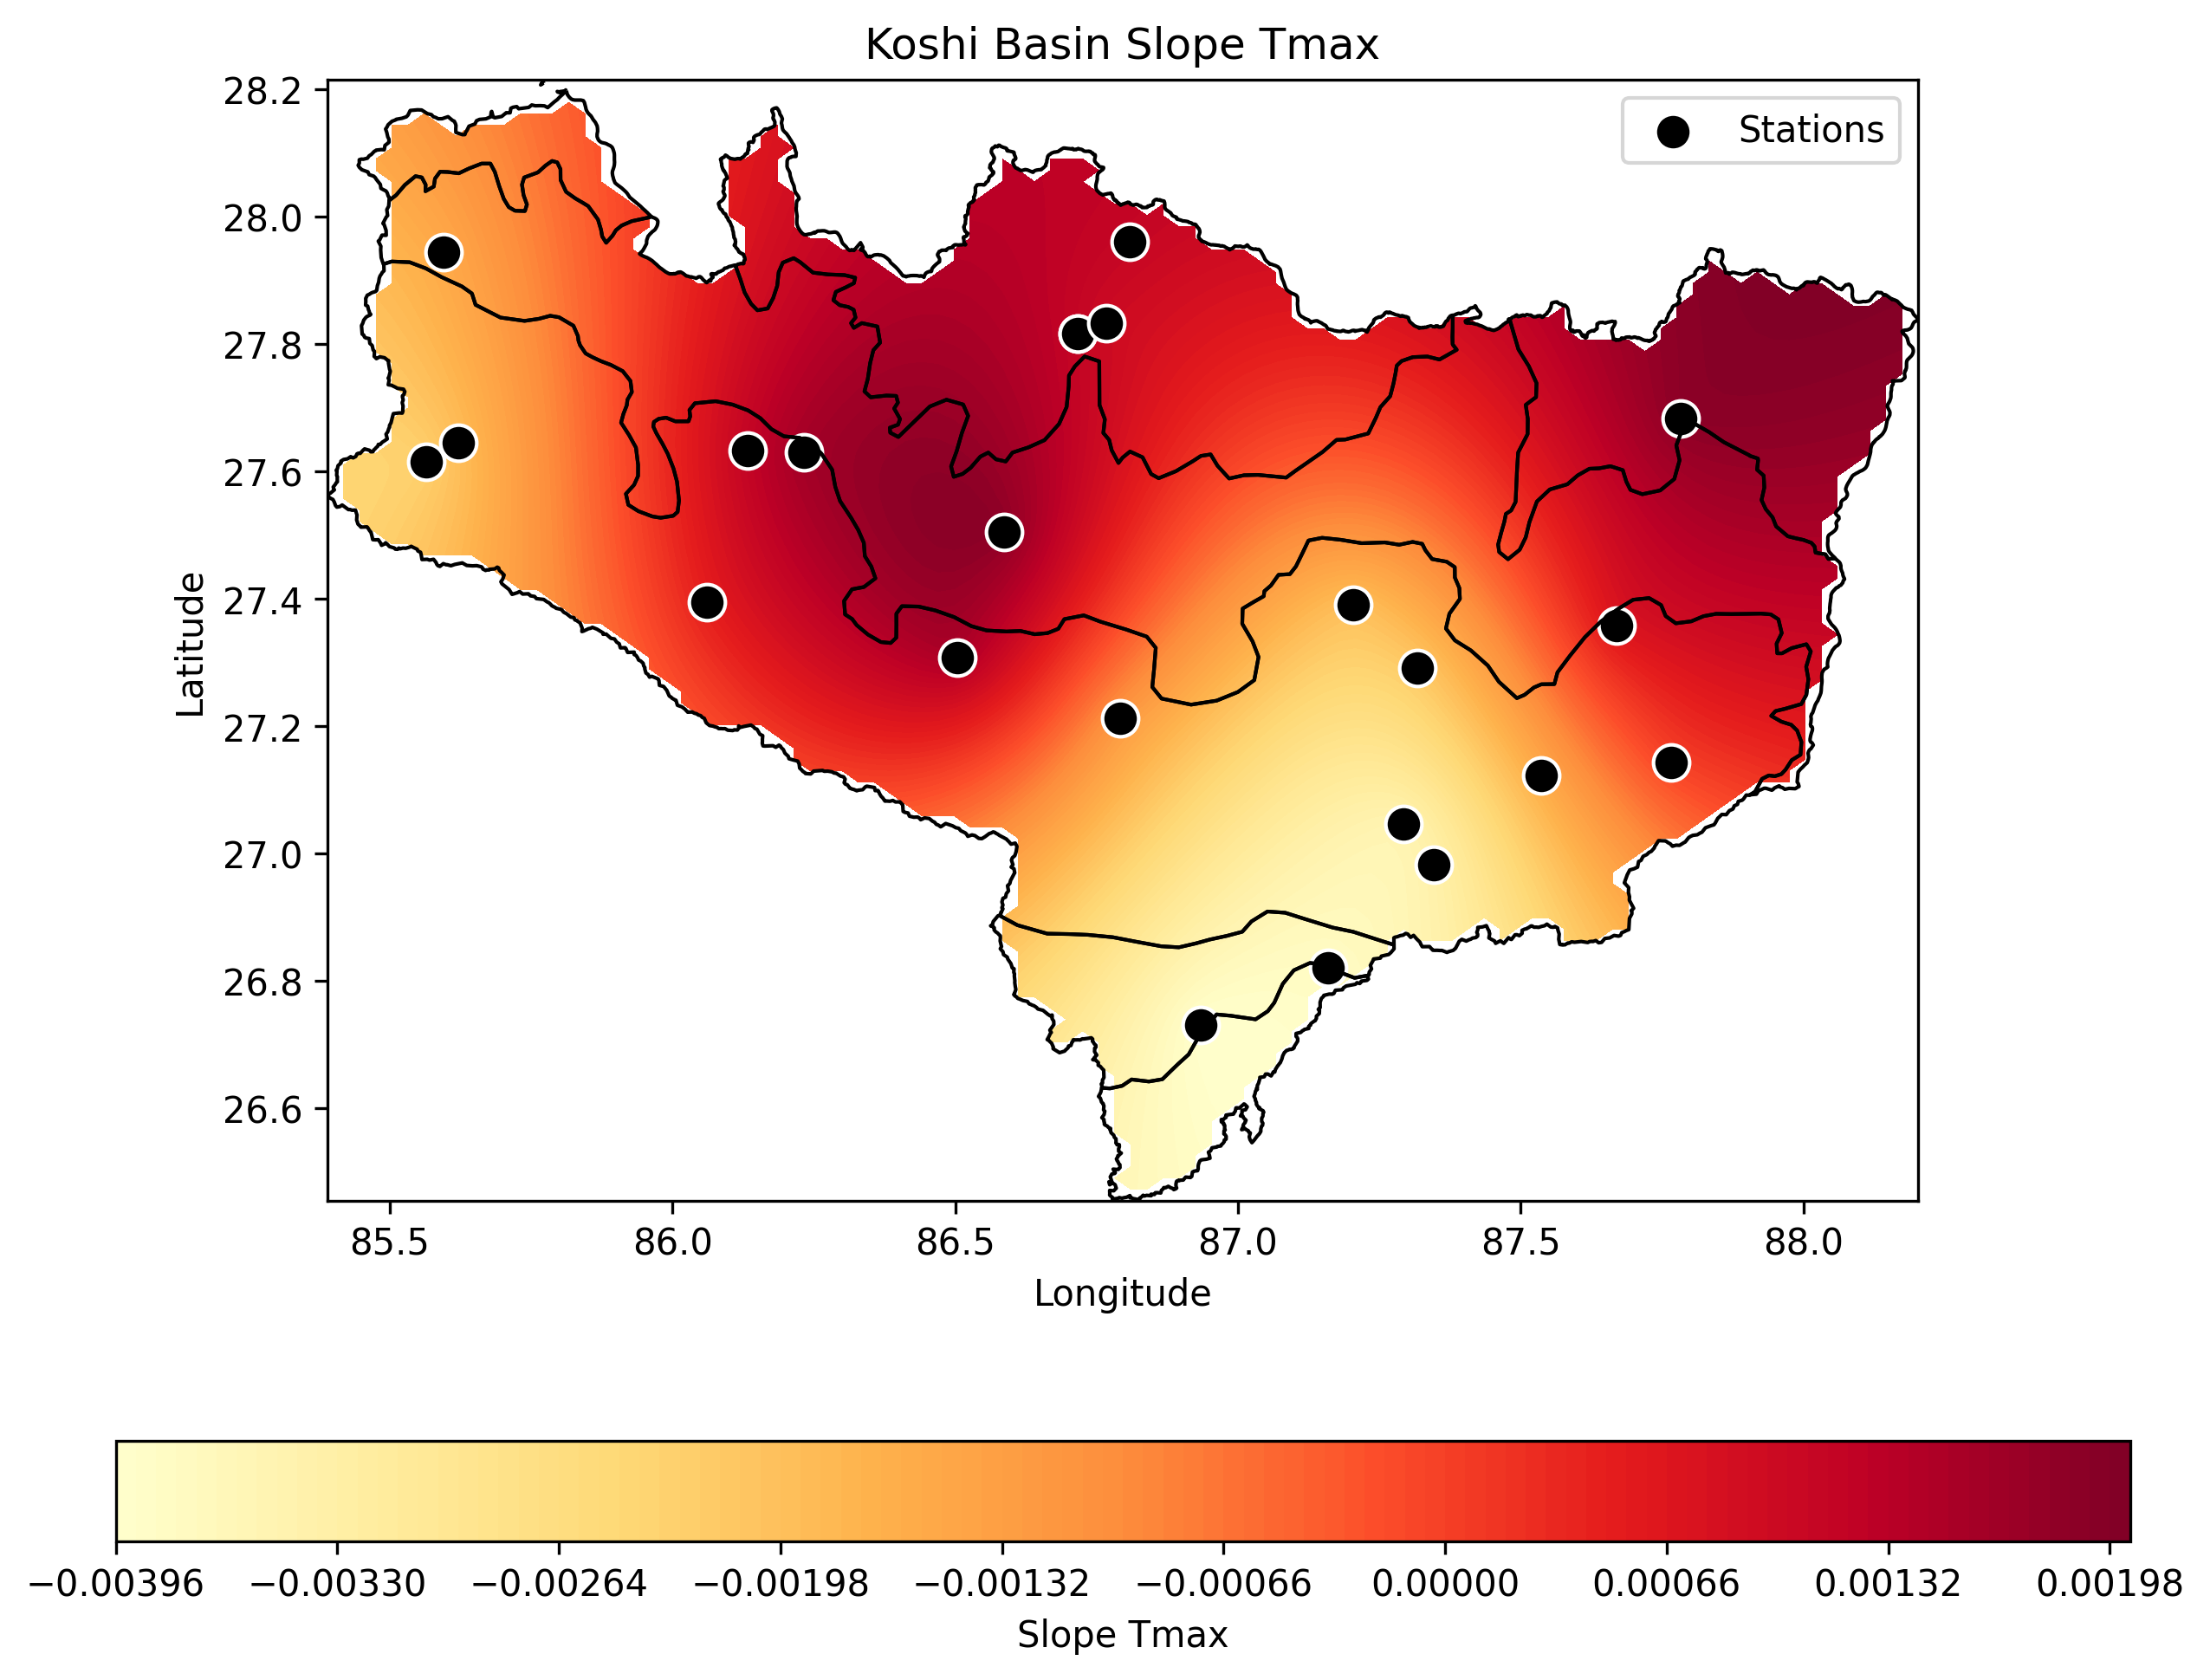
\includegraphics[width=\linewidth]{figure2.png}
        \caption{Caption for subfigure (b)}
        \label{fig:7b}
    \end{subfigure}
    
    \vspace{0.5cm} % Adjust space between rows as needed
    
    \begin{subfigure}{0.45\textwidth}
        \centering
        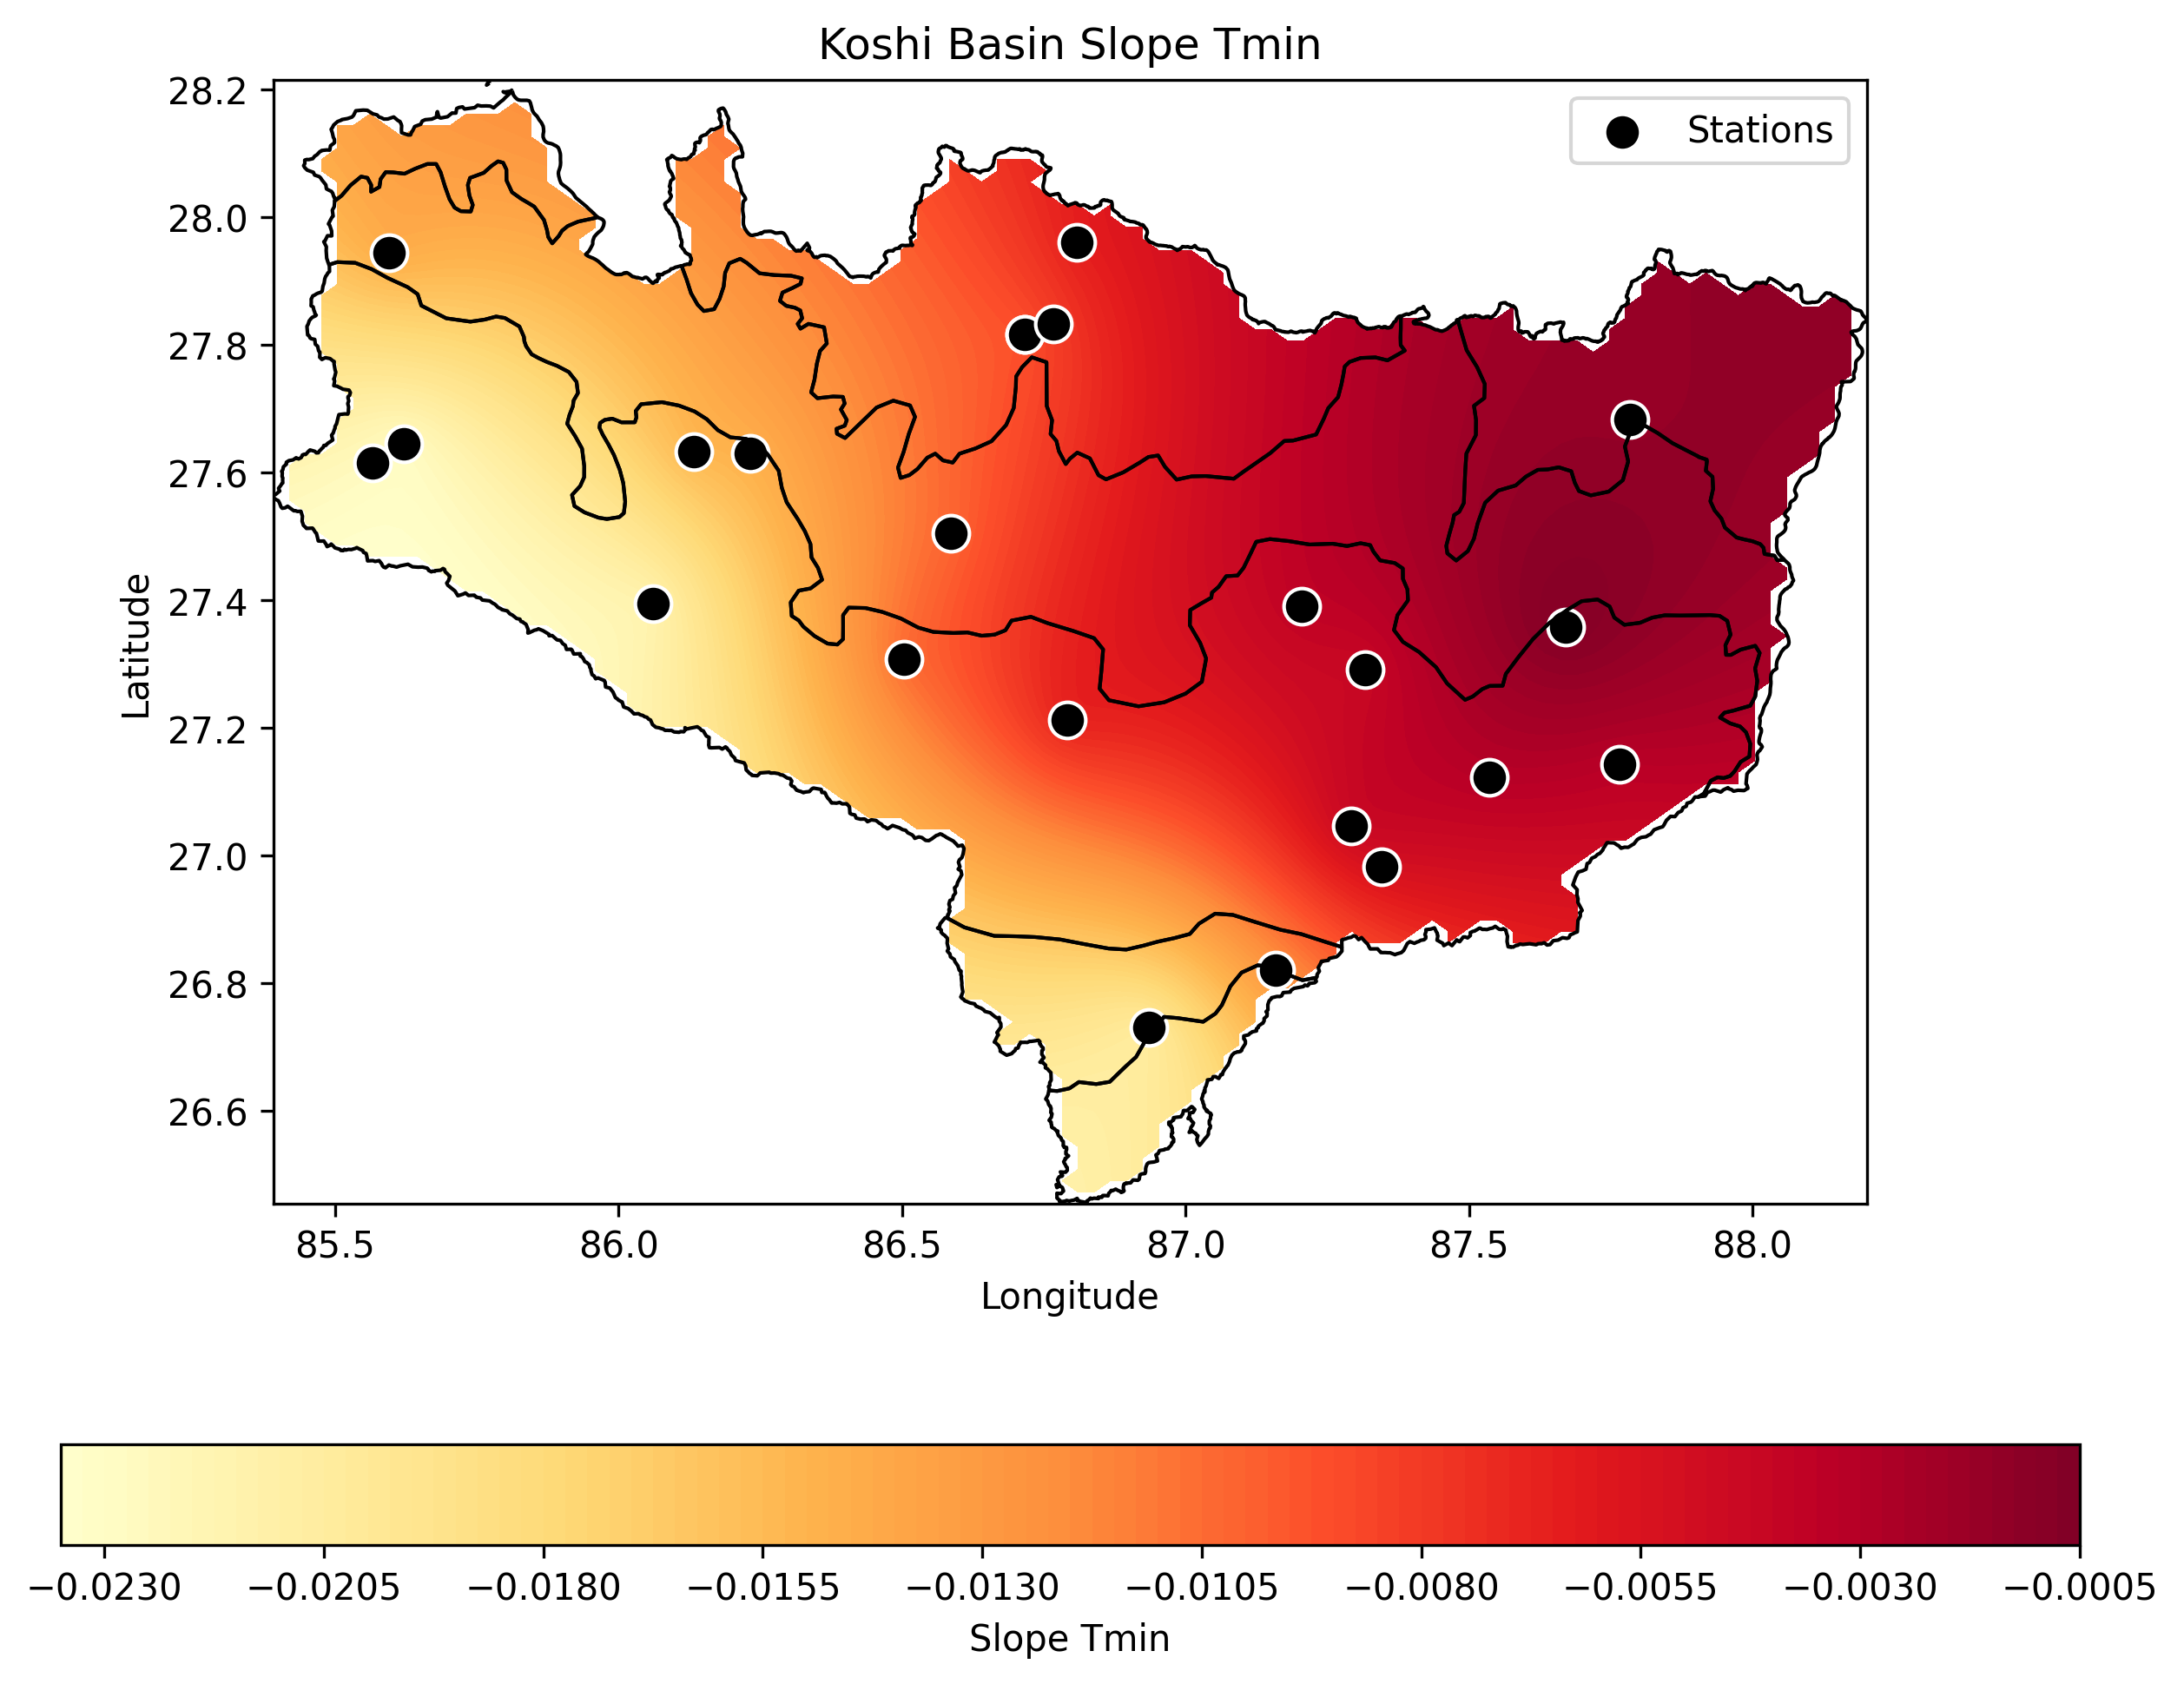
\includegraphics[width=\linewidth]{figure3.png}
        \caption{Caption for subfigure (c)}
        \label{fig:7c}
    \end{subfigure}
    
    \caption{Overall caption for Figure 7, showing subfigures (a), (b), and (c)}
    \label{fig:7}
\end{figure}

\end{document}
